% !TEX root = main.tex
\section{The experiments}
In this section we now describe the two experiments we conducted. They both consists of an iPad application in which the user is told to interact with a balloon on the screen. The iPad choice has been determined by the will of keeping the interaction as natural as possible in order not to make it influent over the measurement of the synchronization aspects of the experiment; the touch interaction on an iPad screen seemed to be the best choice.

We conducted the experiments both with and without a background soundtrack with the intent of understanding the impact of the soundtrack on the task.
\todo[inline]{Expand the soundtrack paragraph. Maybe move this to a separate subsection}

Let us now present the two different experiments in details.

\subsection{\testfirst}
\label{sec:test1}
The first test consisted of an application where the user was asked to tap a red balloon present on the screen. In Figure~\ref{fig:test1} is shown an in-game screen shot of the application.

Every time the user taped on the balloon, this instantaneously moved to a different random location on the screen. The result of such an interaction is the user chasing the balloon around the screen, repeatedly tapping on it. This went on for 60 seconds \todo{Sure?}, we then recorded the sequence of taps on the balloon for every user.

It's worthy of notice the fact that in this experiment the user had no specific goal if not the one of pressing the button. Moreover they were not aware of the duration of the experiment.

This represents a significant difference w.r.t. the second experiment (presented in Section~\ref{sec:test1}), as we will discuss later on.

\begin{figure}[h!t]
\label{fig:test1}
\centering
	{\setlength{\fboxsep}{0pt}
	 \fbox{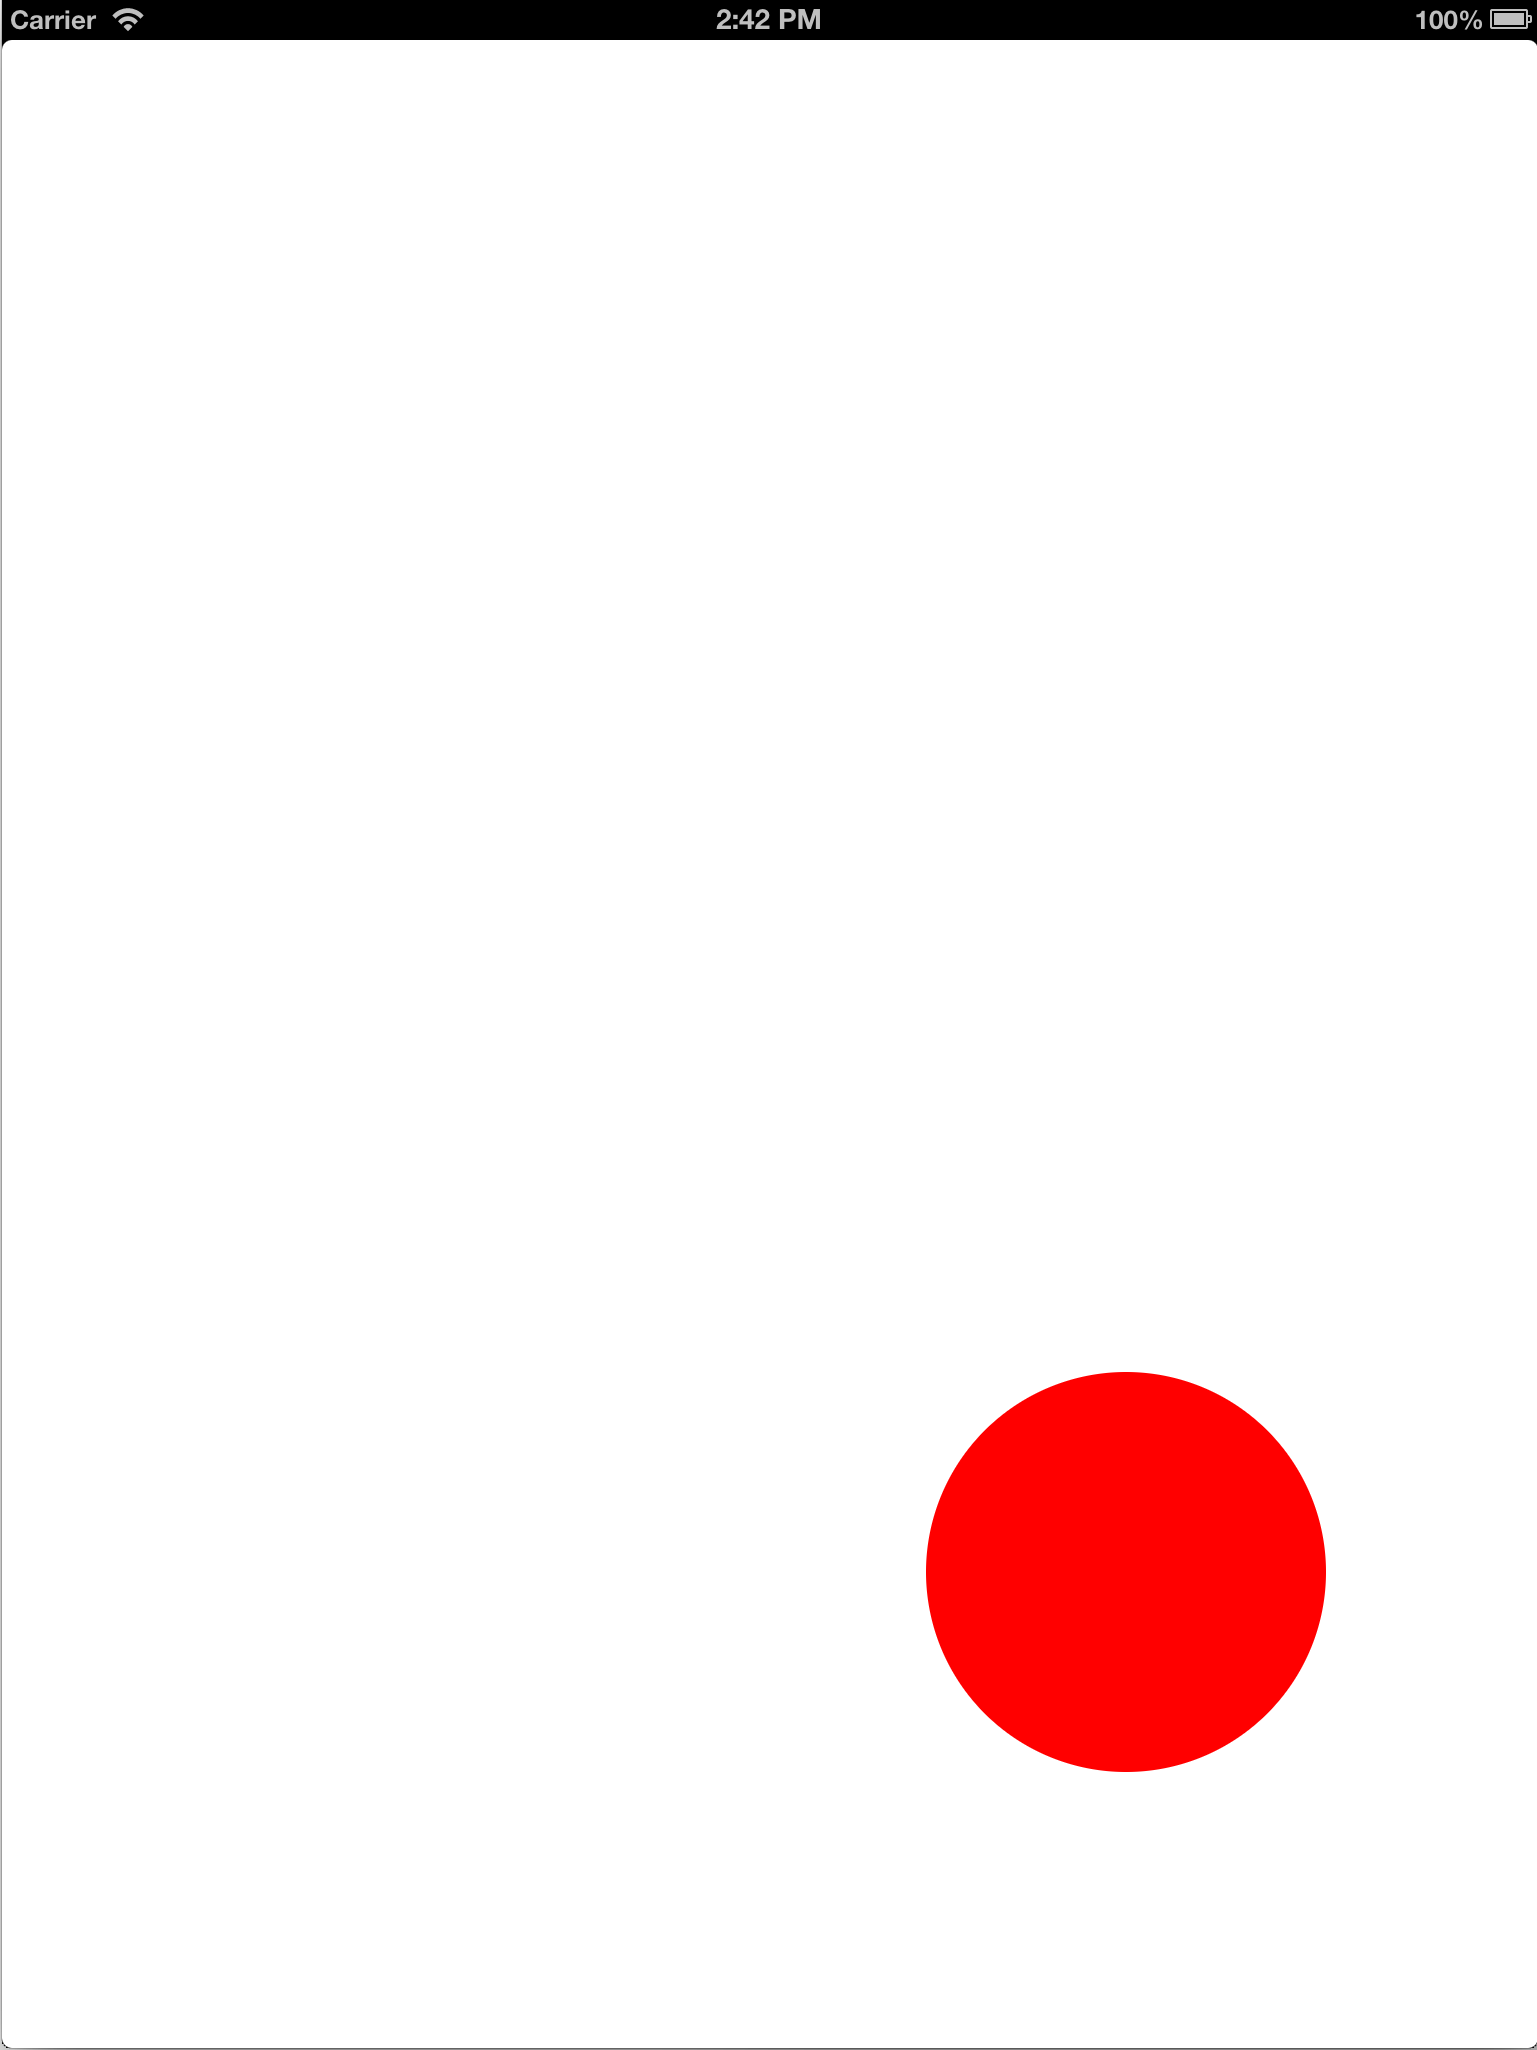
\includegraphics[width=0.45\textwidth]{test1}}}
\caption{\testfirst: in-game screenshot}
\end{figure}

\subsection{Balloon inflater}
\label{sec:test2}
\missingfigure{The second test}
{\color{Gray}{\lipsum[7-15]}}